% This Template is based on the Proposal Template by Constantin Scheuermann and Jan Ole Johanßen. Thanks!

\documentclass[a4paper]{article}

% Define page margine
\usepackage[left=2.5cm,right=2.5cm,top=2.5cm,bottom=2.5cm]{geometry}

% Enable use of figures
\usepackage[pdftex]{graphicx}
\usepackage{float}
\usepackage{floatflt}
\usepackage{enumitem}

% Set line spacing
\usepackage{setspace}
\linespread{1.2}

% Allow for hyphenation
\usepackage{hyphenat}
\hyphenation{over-view}

% Include url package
\usepackage{url}

% Scenarios
\usepackage{longtable}

\title{
%TODO Insert the proposed title
(title) \\
%TODO Insert the proposal type: [Guided Research, Bachelor's Thesis, Master's Thesis, Research Proposal] and number of credits
\small{(Bachelor/Master)'s Thesis (XX ECTS)} \\
%TODO Insert your field of studies
\small{(field of studies)}}

\author{
Supervisor: Prof. Dr.  XY\\
Advisor: XY, M.Sc.\\
%TODO Insert your name
Author: (name)
}

\begin{document}

\maketitle

\begin{abstract}
The abstract summarizes your research project and serves as an overview of the following sections of your proposals.
The reader should be able to instantly understand the problem and get an idea of how you are planning to solve it.

Ideally, an abstract covers the following aspects and is structured accordingly:

\begin{itemize}
	\item \textbf{Motivation/Objective:} Why are you going study the problem? 
	\item \textbf{Problem Statement:} What problem are your trying to solve? 
	\item \textbf{Proposed Solution:} How do you want to tackle the problem? 
	\item \textbf{Approach:} How will you conduct your research?
	\item \textbf{(Expected) Results:} What are the expected results of your research? 
	\item \textbf{Conclusion:}What are your conclusions? 
\end{itemize}

The motivation and objective can be completed by a preamble which introduces the problem domain and facilitates the decision whether the topic is interesting for the reader or not.
A motivation should answer the following questions: why now?
Materials and methods are part of the approach and describe how you accomplished your task.
The result answers the ''what?'' of your written work.
The conclusion summarizes your work.

The proposal serves as a guideline for your advisor as well as for you.
Writing the document is helpful to get a common understanding of the research project.
You can reuse the abstract and proposal as a starting point for your written thesis.\\

\noindent \textbf{Note:} Do not use citations in the abstract! \\ 

\end{abstract}

\newpage

% TODO Remove this section after reading

\section*{Template Information}

This Template is based on the Proposal Template by Constantin Scheuermann and Jan Ole Johanßen. Thanks!

Your research proposal is a short and condensed, yet in some aspects open and incomplete version of your thesis and must be written before you start your (thesis) project.
Therefore, it does not include research results, a detailed requirements elicitation, analysis, or system design and does not contain an object design or implementation details either.

The following chapter represents the structure of a research proposal. 
Each of the following sections contains a short description of the desired content. Replace their content with your text.

\newpage

%TODO Replace the content of the following (sub)sections with your text

\section{Problem Statement}

Describe the problem you want to address and describe why it is a problem.
Start with the problem on a very high level.
Keep your descriptions \textbf{technology independent}.
In other words, depict higher concepts and skip concrete implementation details.

In software engineering terminology, you search for super classes instead of identifying their instances.
For example, \textit{Continuous Integration Service} should be used instead of Bamboo.
Likewise, MQTT is a specific protocol implementation and should be replaced with a \textit{publish/subscribe communication mechanism}.
Keeping a high level of abstraction from the start helps you to generalize the problem.

\section{Proposed Solution}

Formulate your proposed solution based on the problem statement as described in the section before.
Again, keep your explanations technology independent, while giving first hints regarding the solution domain, for example by referring to architectural styles and first ideas on how to tackle the problem.

\section{Related Work}

What is the research context, the theoretical background as well as the state of the art in your field of research?
Are there similar research approaches?
Why is your approach or solution better?
Cite relevant literature and summarize them briefly.

Beside obvious related work, also refer to literature that enabled your topic to define the scope of your work.
What has changed in the past years?
What technology has been introduced?
What has changed in society that the topic is now relevant?
Did a new research fields emerged?

Citations are an important part of this section.
Computer science related papers can be found in the ACM Digital Library\footnote{\url{http://dl.acm.org}, accessed on July 17, 2017} or in the IEEE Xplore Digital Library\footnote{\url{http://ieeexplore.ieee.org}, accessed on July 17, 2017}.
Further, Google Scholar\footnote{\url{https://scholar.google.com}, accessed on July 17, 2017} serves as a good starting point for you initial research.
Use the \verb+footnote+ command to add internet links.
Include the author names in the discussion of related work, such as ''In their paper ABC, Bruegge et al. propose a framework ... [1]''.

\section{Research Approach and Methodology}

Describe your research approach and your methods. Explain how you want to address the problem you described earlier. You can already define a first hypothesis such as: "Automated Delivery in early requirements engineering improve the amount of user involvement.".

\subsection{Research Approach} 

The following selection should help you select your research approach and methodology.
 Sometimes you will follow multiple approaches/methodologies.
 
\begin{itemize}
\item  \textbf{Empirical vs. Non-empirical}: Empirical means to gather experiences about the reality and to order them in a kind of semantic. All steps will be documented, are comprehensible and can be repeated.
Non-empirical research focuses on understanding single topics, using common scientific knowledge in combination with theoretical scientific knowledge. It can be considered a theoretical research \cite{hans2005methoden}.

\item \textbf{Qualitative vs. Quantitative}: A qualitative research approach can be defined as exploratory research using methods such as observation, surveys or questionnaires. Qualitative methods are mostly used in social sciences to observe human behavior. Quantitative research focuses on the systematic empirical investigation of a topic or phenomena. Typically, computation techniques are used. Normally, quantities are \textbf{measured} such as data throughput, time or the amount of something.

\end{itemize}

\subsection{Research Methodology}

In this subsection we introduce some common research methodologies. The list is not comprehensive and the explanations given are not complete. \\

\begin{itemize}
\item \textbf{Conceptional Analysis:} You will investigate on a single question such as 'what is knowledge?' or 'what is a Continuous Delivery'? 
\item \textbf{Concept Implementation:} You will implement an approach you consider to be promising. It focuses on the implementation and its implementation details.
\item \textbf{Case Study:} It is an empirical research methodology, that implements and analyses a phenomenon considering its real-life context.
\item \textbf{Literature Review:} You conduct a structured literature review, categorizing, analyzing and comparing literature in your field of interest. 
\item \textbf{Simulation:} You simulate an algorithm or an approach. During the simulation you are able to control all the dependent variables (as well as the independent).
\item \textbf{Laboratory Experiment:} A laboratory experiment typically includes humans to test a specific design or prototype. You need to take care about the internal and external validity as well as the structure of your experiment and the sample method. The sample method has direct impact if your results are representative or not. Sometimes you just want to provide anecdotal evidence. Internal validity is typically good to control, external validity is challenging.
\item \textbf{Field Experiment:} Same as the laboratory experiment with one major difference: It takes place in the field. You typically are not able to control all the influencing factors, as in a laboratory experiments. Internal validity is difficult to control, while external validity can be considered high. 
\item \textbf{Questionnaire:} Empirical research method using items to gain knowledge about certain research questions or hypothesis. 
\item \textbf{Interview:} Empirical research methodology where you have to have a face to face interview. You ask questions about the topic of interest. Expert interviews are a common interview type.

\end{itemize}


\section{System Requirements and Top Level Design}

Whether you implement a piece of software or you define a process:
Describe your requirements briefly.
Maybe use an scenario.

Then focus on your intended system design.
Again, stay on a high level and be technology independent.
You can either use a textual description or sketch a Top Level Design as shown in \ref{fig:top-level-design}.

\begin{figure}[h]
	\centering
	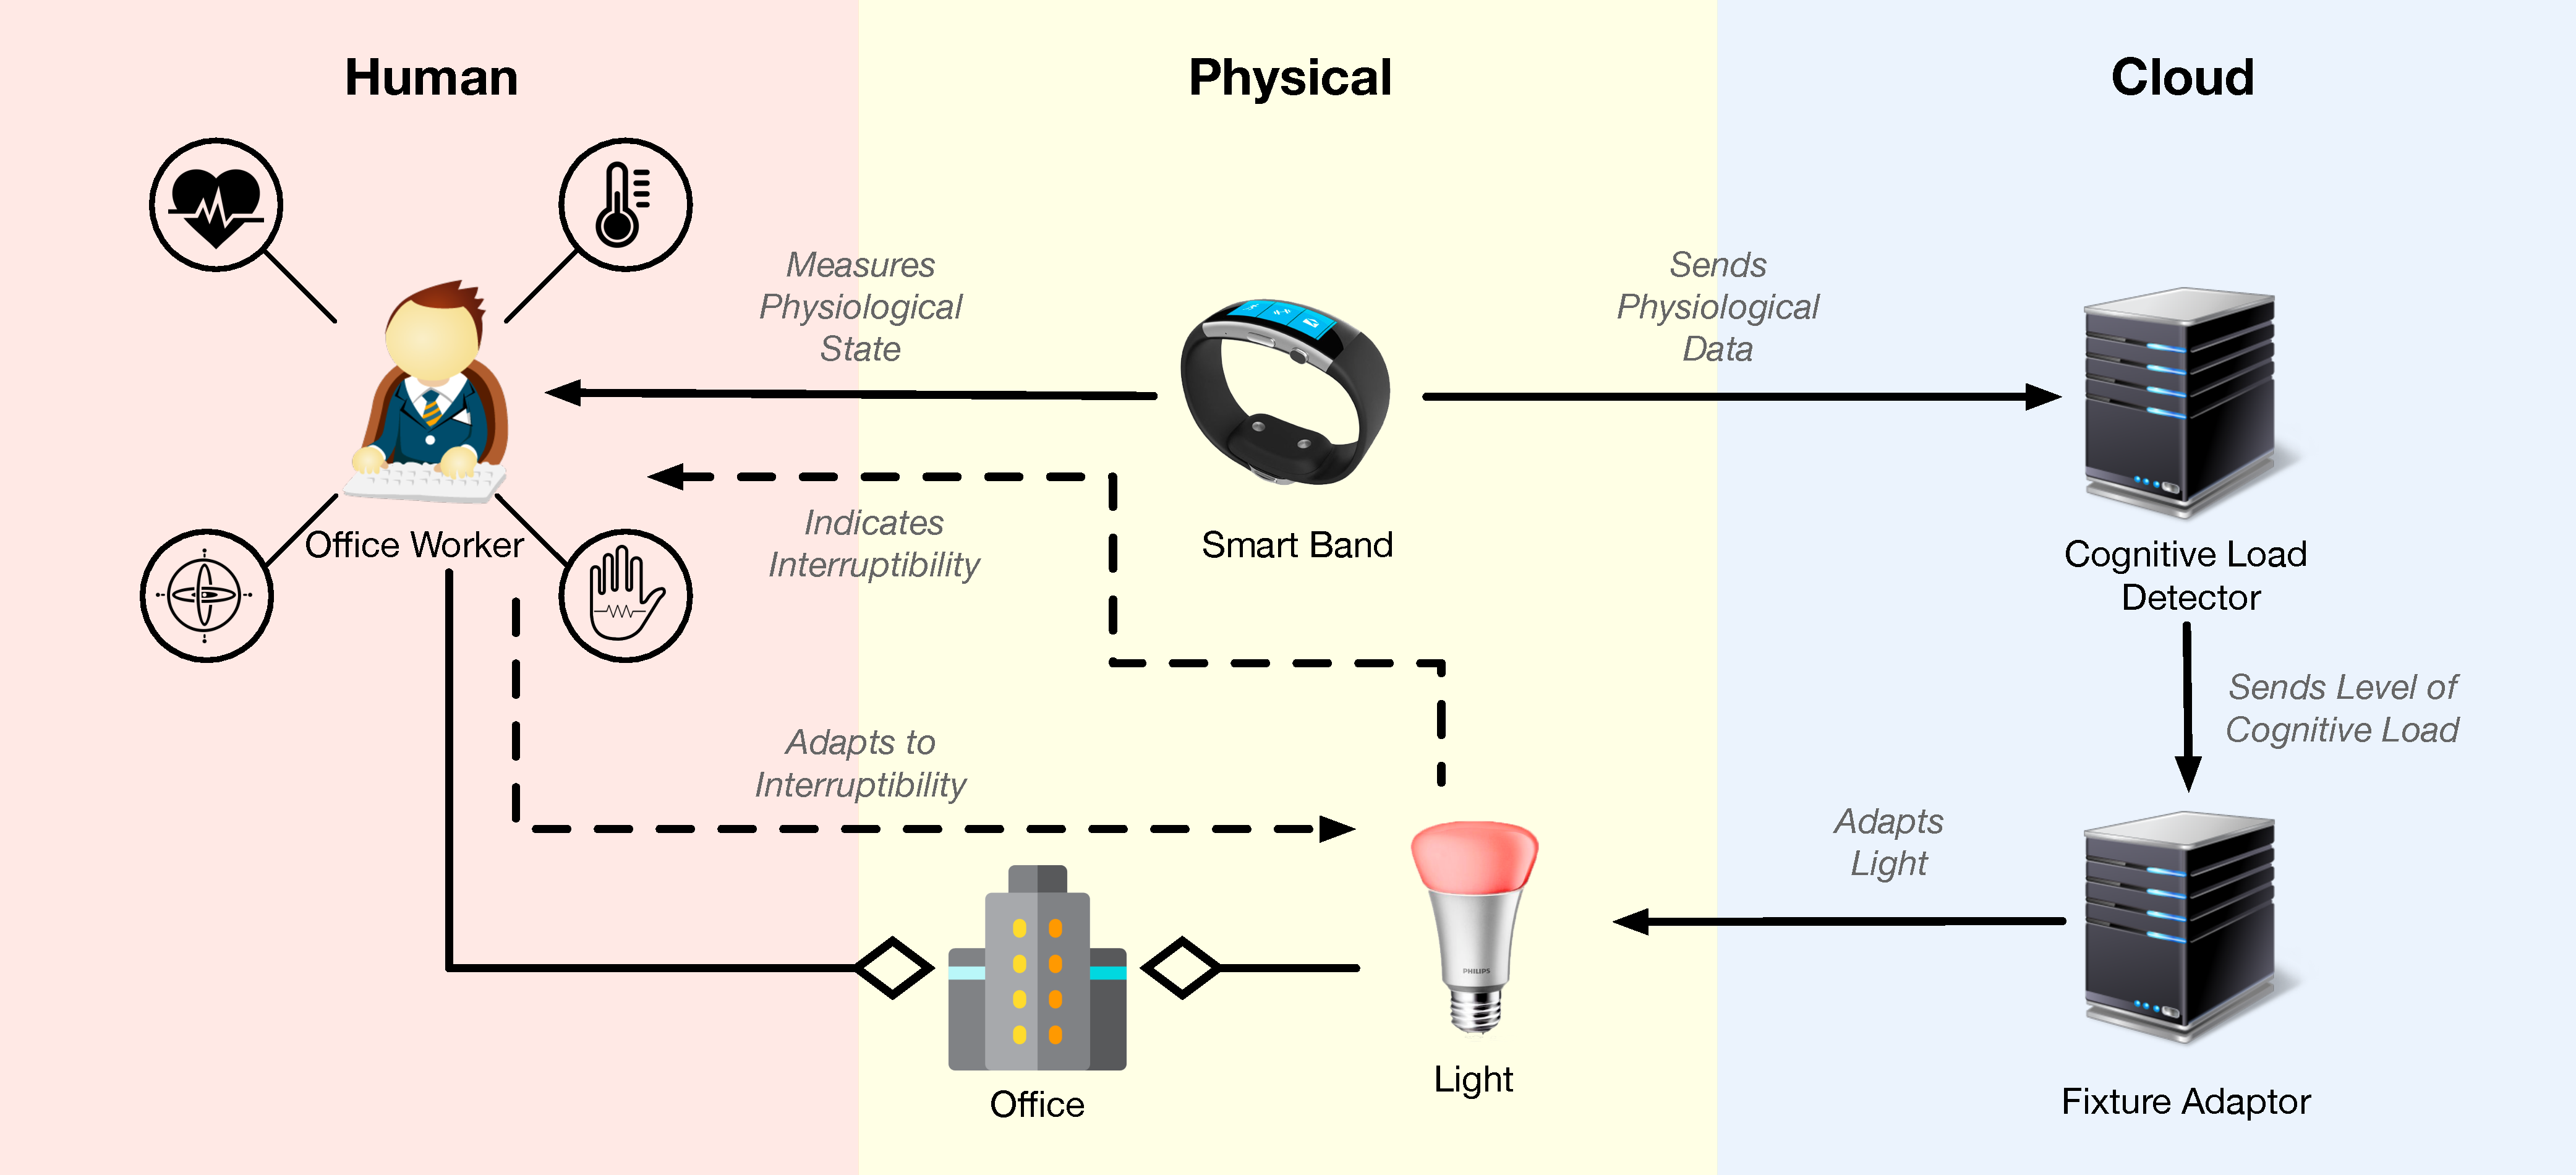
\includegraphics[width=\textwidth]{top-level-design.pdf}
	\caption{Depicting the Top Level Design of the Proposed Sysstem}
	\label{fig:top-level-design}
\end{figure}

\section{Expected Findings}

Write down your expected findings, such as "in this research project we are trying to find out which Iterative Closest Point (ICP) algorithm is most applicable for industrial scene analysis. We expect to get a quantitative ...".
Your expected findings can described on a high level.
However, in case you can provide details, mention them here.

\section*{Time Schedule}
Start by stating the main time points upfront:

\begin{itemize}
	%TODO Update Timeframe
	\item Timeframe: August 15 to February 15, 2017
	%TODO Use the subsequent line in case you (partially) write your thesis abroad, otherwise, skip this addition
	\item Time in Pittsburgh: July 1 to November 15, 2015
\end{itemize}

Then, prepare a brief time schedule with the major milestones.
This is a good basis for discussing your progress with your advisor.
They can quickly see how you understood the concepts and estimated the time effort for your research.
It will serve as guideline during your entire research project.

You can organize your time schedule using a bullet list and stating your most important milestones on a monthly or weekly level:
\begin{itemize}
\item June
	\begin{itemize}
	\item 1\textsuperscript{st} week: Literature research
	\item 2\textsuperscript{nd} week: Infrastructure inspection
	\end{itemize}
\end{itemize}

\noindent Furthermore, in case your research activities are (partially) located abroad, indicate where you plan to work on which work packages.

\end{document}
